\documentclass[twoside]{book}

% Packages required by doxygen
\usepackage{fixltx2e}
\usepackage{calc}
\usepackage{doxygen}
\usepackage[export]{adjustbox} % also loads graphicx
\usepackage{graphicx}
\usepackage[utf8]{inputenc}
\usepackage{makeidx}
\usepackage{multicol}
\usepackage{multirow}
\PassOptionsToPackage{warn}{textcomp}
\usepackage{textcomp}
\usepackage[nointegrals]{wasysym}
\usepackage[table]{xcolor}

% NLS support packages
\usepackage[T2A]{fontenc}
\usepackage[russian]{babel}

% Font selection
\usepackage[T1]{fontenc}
\usepackage[scaled=.90]{helvet}
\usepackage{courier}
\usepackage{amssymb}
\usepackage{sectsty}
\renewcommand{\familydefault}{\sfdefault}
\allsectionsfont{%
  \fontseries{bc}\selectfont%
  \color{darkgray}%
}
\renewcommand{\DoxyLabelFont}{%
  \fontseries{bc}\selectfont%
  \color{darkgray}%
}
\newcommand{\+}{\discretionary{\mbox{\scriptsize$\hookleftarrow$}}{}{}}

% Page & text layout
\usepackage{geometry}
\geometry{%
  a4paper,%
  top=2.5cm,%
  bottom=2.5cm,%
  left=2.5cm,%
  right=2.5cm%
}
\tolerance=750
\hfuzz=15pt
\hbadness=750
\setlength{\emergencystretch}{15pt}
\setlength{\parindent}{0cm}
\setlength{\parskip}{3ex plus 2ex minus 2ex}
\makeatletter
\renewcommand{\paragraph}{%
  \@startsection{paragraph}{4}{0ex}{-1.0ex}{1.0ex}{%
    \normalfont\normalsize\bfseries\SS@parafont%
  }%
}
\renewcommand{\subparagraph}{%
  \@startsection{subparagraph}{5}{0ex}{-1.0ex}{1.0ex}{%
    \normalfont\normalsize\bfseries\SS@subparafont%
  }%
}
\makeatother

% Headers & footers
\usepackage{fancyhdr}
\pagestyle{fancyplain}
\fancyhead[LE]{\fancyplain{}{\bfseries\thepage}}
\fancyhead[CE]{\fancyplain{}{}}
\fancyhead[RE]{\fancyplain{}{\bfseries\leftmark}}
\fancyhead[LO]{\fancyplain{}{\bfseries\rightmark}}
\fancyhead[CO]{\fancyplain{}{}}
\fancyhead[RO]{\fancyplain{}{\bfseries\thepage}}
\fancyfoot[LE]{\fancyplain{}{}}
\fancyfoot[CE]{\fancyplain{}{}}
\fancyfoot[RE]{\fancyplain{}{\bfseries\scriptsize Создано системой Doxygen }}
\fancyfoot[LO]{\fancyplain{}{\bfseries\scriptsize Создано системой Doxygen }}
\fancyfoot[CO]{\fancyplain{}{}}
\fancyfoot[RO]{\fancyplain{}{}}
\renewcommand{\footrulewidth}{0.4pt}
\renewcommand{\chaptermark}[1]{%
  \markboth{#1}{}%
}
\renewcommand{\sectionmark}[1]{%
  \markright{\thesection\ #1}%
}

% Indices & bibliography
\usepackage{natbib}
\usepackage[titles]{tocloft}
\setcounter{tocdepth}{3}
\setcounter{secnumdepth}{5}
\makeindex

% Hyperlinks (required, but should be loaded last)
\usepackage{ifpdf}
\ifpdf
  \usepackage[pdftex,pagebackref=true]{hyperref}
\else
  \usepackage[ps2pdf,pagebackref=true]{hyperref}
\fi
\hypersetup{%
  colorlinks=true,%
  linkcolor=blue,%
  citecolor=blue,%
  unicode%
}

% Custom commands
\newcommand{\clearemptydoublepage}{%
  \newpage{\pagestyle{empty}\cleardoublepage}%
}

\usepackage{caption}
\captionsetup{labelsep=space,justification=centering,font={bf},singlelinecheck=off,skip=4pt,position=top}

%===== C O N T E N T S =====

\begin{document}

% Titlepage & ToC
\hypersetup{pageanchor=false,
             bookmarksnumbered=true,
             pdfencoding=unicode
            }
\pagenumbering{alph}
\begin{titlepage}
\vspace*{7cm}
\begin{center}%
{\Large Isofc for Arm\+Bian }\\
\vspace*{1cm}
{\large Создано системой Doxygen 1.8.14}\\
\end{center}
\end{titlepage}
\clearemptydoublepage
\pagenumbering{roman}
\tableofcontents
\clearemptydoublepage
\pagenumbering{arabic}
\hypersetup{pageanchor=true}

%--- Begin generated contents ---
\chapter{I\+S\+O\+FC for Arm\+Bian}
\label{md_README}
\Hypertarget{md_README}
S\+O\+FT for Arabian\+: The system of secure and authorized exchange of files between the usb device and Samba server

Designed for use in educational organization and enterprises where used and irect mount and use U\+SB drives is prohibit prohibited because of information security requirements.

For autintication of U\+SB drive isofc use a hash file containing the serial number of the U\+SB drive, user login and password

This product is a service that must be constantly running on a computer with access to the S\+A\+M\+BA server

Author\+: Klementyev Mikhail \href{mailto:jollheef@riseup.net}{\tt jollheef@riseup.\+net}

Porting for armbian\+: Nicolskiy Anton \href{mailto:angeloffree@yandex.ru}{\tt angeloffree@yandex.\+ru}

\subsubsection*{Installing on deb based Linux OS}

\begin{DoxyVerb}$ sudo apt install git python3 python3-pip samba samba-common python-glade2 system-config-samba
$ sudo service smbd restart
$ sudo pip3 install pyudev time simplejson configparser
$ git clone https://github.com/OlenEnkeli/isofc_armbian
\end{DoxyVerb}


\subsubsection*{Installing on rpm based Linux OS}

\begin{DoxyVerb}$ sudo rpm install git python3 python3-pip samba samba-client samba-common
$ sudo systemctl restart smb
$ sudo pip3 install pyudev time simplejson configparser
$ git clone https://github.com/OlenEnkeli/isofc_armbian
\end{DoxyVerb}


\subsubsection*{Установка на arch based системах}

\begin{DoxyVerb}$ sudo pacman -S git python python-pip samba
$ sudo systemctl restart smbd
$ sudo pip3 install pyudev time simplejson configparser
$ git clone https://github.com/OlenEnkeli/isofc_armbian
\end{DoxyVerb}


Don\`{}t forget change configuration file and generate open and privacy R\+SA keys

Net you will start ./isofc-\/service.py from cron or another way. 
\chapter{Иерархический список классов}
\section{Иерархия классов}
Иерархия классов.\begin{DoxyCompactList}
\item \contentsline{section}{isofc-\/service.Samba\+Connect}{\pageref{classisofc-service_1_1SambaConnect}}{}
\item Thread\begin{DoxyCompactList}
\item \contentsline{section}{isofc-\/service.Device\+Handler}{\pageref{classisofc-service_1_1DeviceHandler}}{}
\end{DoxyCompactList}
\end{DoxyCompactList}

\chapter{Алфавитный указатель классов}
\section{Классы}
Классы с их кратким описанием.\begin{DoxyCompactList}
\item\contentsline{section}{\mbox{\hyperlink{classisofc-service_1_1DeviceHandler}{isofc-\/service.\+Device\+Handler}} \\*Класс обработки U\+S\+B-\/устройств }{\pageref{classisofc-service_1_1DeviceHandler}}{}
\item\contentsline{section}{\mbox{\hyperlink{classisofc-service_1_1SambaConnect}{isofc-\/service.\+Samba\+Connect}} \\*Класс, выполняющий работу с Samba сервером и синхронизацию файлов }{\pageref{classisofc-service_1_1SambaConnect}}{}
\end{DoxyCompactList}

\chapter{Классы}
\hypertarget{classisofc-service_1_1DeviceHandler}{}\section{Класс isofc-\/service.Device\+Handler}
\label{classisofc-service_1_1DeviceHandler}\index{isofc-\/service.\+Device\+Handler@{isofc-\/service.\+Device\+Handler}}


Класс обработки U\+S\+B-\/устройств  


Граф наследования\+:isofc-\/service.Device\+Handler\+:\begin{figure}[H]
\begin{center}
\leavevmode
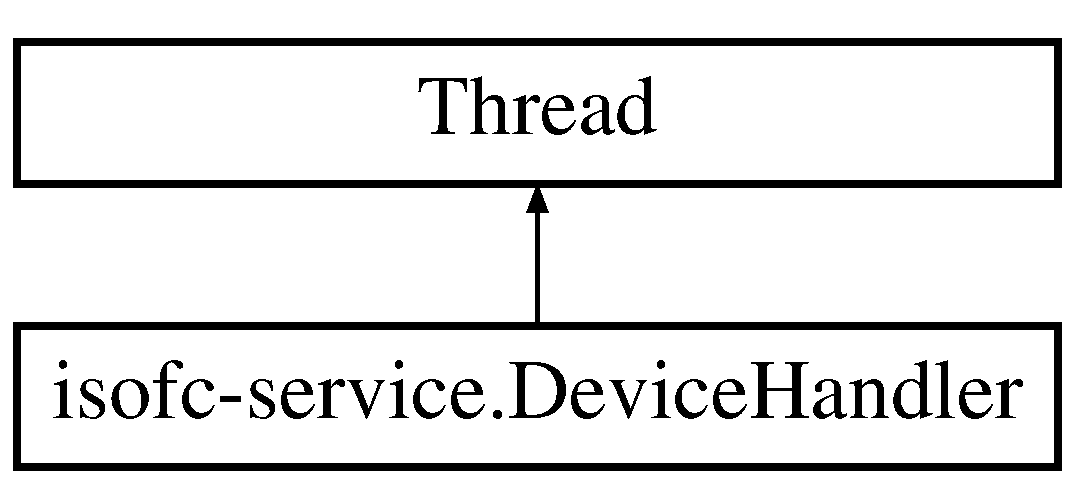
\includegraphics[height=2.000000cm]{classisofc-service_1_1DeviceHandler}
\end{center}
\end{figure}
\subsection*{Открытые члены}
\begin{DoxyCompactItemize}
\item 
\mbox{\Hypertarget{classisofc-service_1_1DeviceHandler_af953fc36e5e72bc5ef726f7438878253}\label{classisofc-service_1_1DeviceHandler_af953fc36e5e72bc5ef726f7438878253}} 
def {\bfseries \+\_\+\+\_\+init\+\_\+\+\_\+} (self)
\item 
\mbox{\Hypertarget{classisofc-service_1_1DeviceHandler_a76c4196af1b16fc1bdec00f97500516e}\label{classisofc-service_1_1DeviceHandler_a76c4196af1b16fc1bdec00f97500516e}} 
def {\bfseries run} (self)
\item 
def \mbox{\hyperlink{classisofc-service_1_1DeviceHandler_a87ac1ab9b3b6658023374dd42299acec}{Run\+Monitor}} (self)
\begin{DoxyCompactList}\small\item\em Функция, запускающая обработка мониторинга подключения U\+SB устройств к системе \end{DoxyCompactList}\item 
\mbox{\Hypertarget{classisofc-service_1_1DeviceHandler_ac095965e3237db7b074f7b84a552e0b9}\label{classisofc-service_1_1DeviceHandler_ac095965e3237db7b074f7b84a552e0b9}} 
def {\bfseries Run\+Thread} (self, action, device)
\item 
def \mbox{\hyperlink{classisofc-service_1_1DeviceHandler_ac3913ebd2f7446cdaa3242cc10215bb0}{Check\+Auth}} (self, device, usbdirectory)
\begin{DoxyCompactList}\small\item\em Функция проверки аутефикации на Samba-\/сервере \end{DoxyCompactList}\item 
def \mbox{\hyperlink{classisofc-service_1_1DeviceHandler_a3a5203ad41382b069d77e6fa783253fc}{Decrypt}} (self, ciphertext)
\begin{DoxyCompactList}\small\item\em Функция расшифровки файла с данными авторизации \end{DoxyCompactList}\item 
def \mbox{\hyperlink{classisofc-service_1_1DeviceHandler_a1fac2973c2340523f8640b56974574cb}{Usb\+Mount}} (self, device)
\begin{DoxyCompactList}\small\item\em Функция монтирования usb. \end{DoxyCompactList}\item 
def \mbox{\hyperlink{classisofc-service_1_1DeviceHandler_aaaa9fa346a748b4acded6cc698cd5c31}{Usb\+Umount}} (self, device)
\begin{DoxyCompactList}\small\item\em Функция размонтирования usb. \end{DoxyCompactList}\item 
def \mbox{\hyperlink{classisofc-service_1_1DeviceHandler_ace0b9c671ec50f9e343a2ab3dc39203e}{Handle}} (self, action, device)
\begin{DoxyCompactList}\small\item\em Функция обработки состояний U\+SB устройства \end{DoxyCompactList}\end{DoxyCompactItemize}
\subsection*{Открытые атрибуты}
\begin{DoxyCompactItemize}
\item 
\mbox{\Hypertarget{classisofc-service_1_1DeviceHandler_aca19cb30a27a1352836b3fe6dfa9d347}\label{classisofc-service_1_1DeviceHandler_aca19cb30a27a1352836b3fe6dfa9d347}} 
{\bfseries quit}
\item 
\mbox{\Hypertarget{classisofc-service_1_1DeviceHandler_a924f7fb2ce60b6d7c0cf1ae12f8c99f7}\label{classisofc-service_1_1DeviceHandler_a924f7fb2ce60b6d7c0cf1ae12f8c99f7}} 
{\bfseries Exit\+Flag}
\item 
\mbox{\Hypertarget{classisofc-service_1_1DeviceHandler_a69d7a83a92fa887dc5455bd624ec6f17}\label{classisofc-service_1_1DeviceHandler_a69d7a83a92fa887dc5455bd624ec6f17}} 
{\bfseries observer}
\end{DoxyCompactItemize}
\subsection*{Статические открытые данные}
\begin{DoxyCompactItemize}
\item 
\mbox{\Hypertarget{classisofc-service_1_1DeviceHandler_a400ab1f0978eacc7cc3bd5d6bac10ca7}\label{classisofc-service_1_1DeviceHandler_a400ab1f0978eacc7cc3bd5d6bac10ca7}} 
bool {\bfseries Exit\+Flag} = False
\item 
dictionary \mbox{\hyperlink{classisofc-service_1_1DeviceHandler_a23d3bade1a4584ff598cfc9bd7cafc8b}{Status\+Msg}}
\begin{DoxyCompactList}\small\item\em Сообщения для вывода на дисплей \end{DoxyCompactList}\end{DoxyCompactItemize}


\subsection{Подробное описание}
Класс обработки U\+S\+B-\/устройств 

\subsection{Методы}
\mbox{\Hypertarget{classisofc-service_1_1DeviceHandler_ac3913ebd2f7446cdaa3242cc10215bb0}\label{classisofc-service_1_1DeviceHandler_ac3913ebd2f7446cdaa3242cc10215bb0}} 
\index{isofc-\/service\+::\+Device\+Handler@{isofc-\/service\+::\+Device\+Handler}!Check\+Auth@{Check\+Auth}}
\index{Check\+Auth@{Check\+Auth}!isofc-\/service\+::\+Device\+Handler@{isofc-\/service\+::\+Device\+Handler}}
\subsubsection{\texorpdfstring{Check\+Auth()}{CheckAuth()}}
{\footnotesize\ttfamily def isofc-\/service.\+Device\+Handler.\+Check\+Auth (\begin{DoxyParamCaption}\item[{}]{self,  }\item[{}]{device,  }\item[{}]{usbdirectory }\end{DoxyParamCaption})}



Функция проверки аутефикации на Samba-\/сервере 

Идет проверка на существование файла ./isofc\+\_\+credentials

Файл расшифровывается, сверяется serial id устройства в usb порте и serial id из файла аутефикации


\begin{DoxyParams}{Аргументы}
{\em ciphertext} & -\/ входная строка (зашифрованный текст) \\
\hline
{\em private\+\_\+key\+\_\+path} & -\/ путь к файлу секретного ключа \\
\hline
{\em opentext} & -\/ расшифрованный текст \\
\hline
\end{DoxyParams}

\begin{DoxyCode}
135     \textcolor{keyword}{def }CheckAuth(self, device, usbdirectory):
136         \textcolor{keywordflow}{try}:
137             f = open(usbdirectory + \textcolor{stringliteral}{"/.isofc\_credentials"}, \textcolor{stringliteral}{"r")}
138 \textcolor{stringliteral}{            data = f.read().replace('\(\backslash\)n'}, \textcolor{stringliteral}{''})
139         \textcolor{keywordflow}{except} IOError \textcolor{keyword}{as} exc:
140             \textcolor{keywordflow}{if} exc.errno == 2:
141                 \textcolor{keywordflow}{return} [\textcolor{keyword}{False}, self.StatusMsg[\textcolor{stringliteral}{'AuthFileNotFoundError'}]] \textcolor{comment}{# Нет файла аутенфикации}
142             \textcolor{keywordflow}{else}:
143                 \textcolor{keywordflow}{return} \textcolor{keywordtype}{None}
144         Credentials = self.Decrypt(data) \textcolor{comment}{# функция расшифровки файла аутенфикации}
145 
146         \textcolor{keywordflow}{if} Credentials == \textcolor{stringliteral}{'Error'}:
147             \textcolor{keywordflow}{return} [\textcolor{keyword}{False}, self.StatusMsg[\textcolor{stringliteral}{'WrongAuthFileError'}]]
148         \textcolor{keywordflow}{try}:
149             Credentials = json.loads(Credentials)
150             serial = device[\textcolor{stringliteral}{'ID\_SERIAL'}]
151         \textcolor{keywordflow}{except}:
152             \textcolor{keywordflow}{return} [\textcolor{keyword}{False}, self.StatusMsg[\textcolor{stringliteral}{'WrongAuthFileError'}]]
153         \textcolor{keywordflow}{if} serial.lower() != Credentials[\textcolor{stringliteral}{'Serial'}].lower():
154             Log(\textcolor{stringliteral}{"Serial ID in credentials ("} + Credentials[\textcolor{stringliteral}{'Serial'}].lower()
155                 + \textcolor{stringliteral}{") is not equal serial ID in usb device ("}
156                 +  serial.lower() + \textcolor{stringliteral}{")"})
157             \textcolor{keywordflow}{return} [\textcolor{keyword}{False}, self.StatusMsg[\textcolor{stringliteral}{'WrongAuthFileError'}]]
158 
159         f.close()
160 
161         \textcolor{keywordflow}{return} [\textcolor{keyword}{True}, Credentials[\textcolor{stringliteral}{'Login'}], Credentials[\textcolor{stringliteral}{'Password'}], serial]
162 
\end{DoxyCode}
\mbox{\Hypertarget{classisofc-service_1_1DeviceHandler_a3a5203ad41382b069d77e6fa783253fc}\label{classisofc-service_1_1DeviceHandler_a3a5203ad41382b069d77e6fa783253fc}} 
\index{isofc-\/service\+::\+Device\+Handler@{isofc-\/service\+::\+Device\+Handler}!Decrypt@{Decrypt}}
\index{Decrypt@{Decrypt}!isofc-\/service\+::\+Device\+Handler@{isofc-\/service\+::\+Device\+Handler}}
\subsubsection{\texorpdfstring{Decrypt()}{Decrypt()}}
{\footnotesize\ttfamily def isofc-\/service.\+Device\+Handler.\+Decrypt (\begin{DoxyParamCaption}\item[{}]{self,  }\item[{}]{ciphertext }\end{DoxyParamCaption})}



Функция расшифровки файла с данными авторизации 

Идет проверка на существование файла секретного ключа.

Файл расшифровывается последовательно base64 -\/$>$ rsa с помошью секретного ключа 
\begin{DoxyParams}{Аргументы}
{\em ciphertext} & -\/ входная строка (зашифрованный текст) \\
\hline
{\em private\+\_\+key\+\_\+path} & -\/ путь к файлу секретного ключа \\
\hline
{\em opentext} & -\/ расшифрованный текст \\
\hline
\end{DoxyParams}

\begin{DoxyCode}
171     \textcolor{keyword}{def }Decrypt(self, ciphertext):
172         \textcolor{keyword}{global} config
173         \textcolor{keywordflow}{if} \textcolor{keywordflow}{not} os.path.isfile(config[\textcolor{stringliteral}{"private\_key\_path"}]):
174             Log(\textcolor{stringliteral}{"Private key not found"})
175             \textcolor{keywordflow}{return} \textcolor{stringliteral}{'Error'}
176         \textcolor{keywordflow}{if} \textcolor{keywordflow}{not} base64p(ciphertext):
177             Log(\textcolor{stringliteral}{".isofc\_credentials is not base64, Ciphertext = '"}
178                 + str(ciphertext) + \textcolor{stringliteral}{"'"})
179             \textcolor{keywordflow}{return} \textcolor{stringliteral}{'Error'}
180         retcode, opentext = getstatusoutput(
181             \textcolor{stringliteral}{"echo "} + ciphertext + \textcolor{stringliteral}{"|base64 -d|openssl rsautl -inkey "}
182             + config[\textcolor{stringliteral}{"private\_key\_path"}] + \textcolor{stringliteral}{" -decrypt"})
183         Log(\textcolor{stringliteral}{"Retcode(decrypt): "} + str(retcode))
184         \textcolor{keywordflow}{if} retcode == 0:
185             \textcolor{keywordflow}{return} opentext
186         \textcolor{keywordflow}{else}:
187             \textcolor{keywordflow}{return} \textcolor{stringliteral}{'Error'}
188 
\end{DoxyCode}
\mbox{\Hypertarget{classisofc-service_1_1DeviceHandler_ace0b9c671ec50f9e343a2ab3dc39203e}\label{classisofc-service_1_1DeviceHandler_ace0b9c671ec50f9e343a2ab3dc39203e}} 
\index{isofc-\/service\+::\+Device\+Handler@{isofc-\/service\+::\+Device\+Handler}!Handle@{Handle}}
\index{Handle@{Handle}!isofc-\/service\+::\+Device\+Handler@{isofc-\/service\+::\+Device\+Handler}}
\subsubsection{\texorpdfstring{Handle()}{Handle()}}
{\footnotesize\ttfamily def isofc-\/service.\+Device\+Handler.\+Handle (\begin{DoxyParamCaption}\item[{}]{self,  }\item[{}]{action,  }\item[{}]{device }\end{DoxyParamCaption})}



Функция обработки состояний U\+SB устройства 


\begin{DoxyParams}{Аргументы}
{\em action} & -\/ действие, произведенное с устройством (add или remove) \\
\hline
\end{DoxyParams}

\begin{DoxyCode}
203     \textcolor{keyword}{def }Handle(self,action,device):
204         \textcolor{keywordflow}{try}:
205             Log(\textcolor{stringliteral}{"Action: "} + str(action) + \textcolor{stringliteral}{", "}
206                 + \textcolor{stringliteral}{"DEVNAME: "} + str(device[\textcolor{stringliteral}{'DEVNAME'}]) + \textcolor{stringliteral}{", "}
207                 + \textcolor{stringliteral}{"ID\_SERIAL: "} + str(device[\textcolor{stringliteral}{'ID\_SERIAL'}]) + \textcolor{stringliteral}{" "})
208         \textcolor{keywordflow}{except}:
209             Log(\textcolor{stringliteral}{"Fail on Port: "} + str(Port(device)) + \textcolor{stringliteral}{", "}
210                 + \textcolor{stringliteral}{"Action: "} + str(action))
211             \textcolor{keywordflow}{return} \textcolor{keywordtype}{None}
212 
213         \textcolor{keywordflow}{if} str(action) == \textcolor{stringliteral}{"add"}:
214             retval, usbdirectory = self.UsbMount(device)
215 
216             \textcolor{keywordflow}{if} retval != 0:
217                 Log(\textcolor{stringliteral}{"Cannot mount "} + str(device.device\_node))
218                 \textcolor{keywordflow}{return} \textcolor{keywordtype}{None}
219 
220             Log(str(device.device\_node) + \textcolor{stringliteral}{" mounted"})
221 
222             Credentials = self.CheckAuth(device, usbdirectory)
223 
224             \textcolor{keywordflow}{if} \textcolor{keywordflow}{not} Credentials[0]:
225                 Log(Credentials[1])
226             \textcolor{keywordflow}{else}:
227                 Log(str(device.device\_node) + \textcolor{stringliteral}{", "}
228                     + \textcolor{stringliteral}{"Login: "} + Credentials[1] + \textcolor{stringliteral}{", "}
229                     + \textcolor{stringliteral}{"Serial: "} + Credentials[3])
230 
231                 smbConnect = SambaConnect(Credentials[1],Credentials[2],device,usbdirectory)
232 
233             \textcolor{keywordflow}{if} self.UsbUmount(device) != 0:
234                 Log(str(device.device\_node) + \textcolor{stringliteral}{", failed umount"})
235                 \textcolor{keywordflow}{return} \textcolor{keywordtype}{None}
236 
237             Log(str(device.device\_node) + \textcolor{stringliteral}{" umounted"})
238 
239         \textcolor{keywordflow}{if} str(action) == \textcolor{stringliteral}{"remove"}:
240             \textcolor{keywordflow}{pass}
241 
\end{DoxyCode}
\mbox{\Hypertarget{classisofc-service_1_1DeviceHandler_a87ac1ab9b3b6658023374dd42299acec}\label{classisofc-service_1_1DeviceHandler_a87ac1ab9b3b6658023374dd42299acec}} 
\index{isofc-\/service\+::\+Device\+Handler@{isofc-\/service\+::\+Device\+Handler}!Run\+Monitor@{Run\+Monitor}}
\index{Run\+Monitor@{Run\+Monitor}!isofc-\/service\+::\+Device\+Handler@{isofc-\/service\+::\+Device\+Handler}}
\subsubsection{\texorpdfstring{Run\+Monitor()}{RunMonitor()}}
{\footnotesize\ttfamily def isofc-\/service.\+Device\+Handler.\+Run\+Monitor (\begin{DoxyParamCaption}\item[{}]{self }\end{DoxyParamCaption})}



Функция, запускающая обработка мониторинга подключения U\+SB устройств к системе 


\begin{DoxyParams}{Аргументы}
{\em self} & -\/ Возвратный указатель \\
\hline
\end{DoxyParams}

\begin{DoxyCode}
110     \textcolor{keyword}{def }RunMonitor(self):
111         context = pyudev.Context()
112         monitor = pyudev.Monitor.from\_netlink(context)
113         monitor.filter\_by(\textcolor{stringliteral}{'block'})
114 
115         \textcolor{comment}{# Вызов монитора udev - для вновь подключенного или отключенного устройства вызывается новый тред}
116         self.observer = pyudev.MonitorObserver(
117             monitor,
118             \textcolor{keyword}{lambda} action,device : self.RunThread(action,device))
119 
\end{DoxyCode}
\mbox{\Hypertarget{classisofc-service_1_1DeviceHandler_a1fac2973c2340523f8640b56974574cb}\label{classisofc-service_1_1DeviceHandler_a1fac2973c2340523f8640b56974574cb}} 
\index{isofc-\/service\+::\+Device\+Handler@{isofc-\/service\+::\+Device\+Handler}!Usb\+Mount@{Usb\+Mount}}
\index{Usb\+Mount@{Usb\+Mount}!isofc-\/service\+::\+Device\+Handler@{isofc-\/service\+::\+Device\+Handler}}
\subsubsection{\texorpdfstring{Usb\+Mount()}{UsbMount()}}
{\footnotesize\ttfamily def isofc-\/service.\+Device\+Handler.\+Usb\+Mount (\begin{DoxyParamCaption}\item[{}]{self,  }\item[{}]{device }\end{DoxyParamCaption})}



Функция монтирования usb. 


\begin{DoxyParams}{Аргументы}
{\em device} & -\/ устройство \\
\hline
\end{DoxyParams}

\begin{DoxyCode}
191     \textcolor{keyword}{def }UsbMount(self,device):
192         retval, output = getstatusoutput(\textcolor{stringliteral}{"pmount "} + device.device\_node)
193         \textcolor{keywordflow}{return} [retval, re.sub(\textcolor{stringliteral}{r'dev'}, \textcolor{stringliteral}{'media'}, device.device\_node)]
194 
\end{DoxyCode}
\mbox{\Hypertarget{classisofc-service_1_1DeviceHandler_aaaa9fa346a748b4acded6cc698cd5c31}\label{classisofc-service_1_1DeviceHandler_aaaa9fa346a748b4acded6cc698cd5c31}} 
\index{isofc-\/service\+::\+Device\+Handler@{isofc-\/service\+::\+Device\+Handler}!Usb\+Umount@{Usb\+Umount}}
\index{Usb\+Umount@{Usb\+Umount}!isofc-\/service\+::\+Device\+Handler@{isofc-\/service\+::\+Device\+Handler}}
\subsubsection{\texorpdfstring{Usb\+Umount()}{UsbUmount()}}
{\footnotesize\ttfamily def isofc-\/service.\+Device\+Handler.\+Usb\+Umount (\begin{DoxyParamCaption}\item[{}]{self,  }\item[{}]{device }\end{DoxyParamCaption})}



Функция размонтирования usb. 


\begin{DoxyParams}{Аргументы}
{\em device} & -\/ устройство \\
\hline
\end{DoxyParams}

\begin{DoxyCode}
197     \textcolor{keyword}{def }UsbUmount(self,device):
198         retval, output = getstatusoutput(\textcolor{stringliteral}{"pumount "} + re.sub(\textcolor{stringliteral}{r'dev'}, \textcolor{stringliteral}{'media'}, device.device\_node))
199         \textcolor{keywordflow}{return} retval
200 
\end{DoxyCode}


\subsection{Данные класса}
\mbox{\Hypertarget{classisofc-service_1_1DeviceHandler_a23d3bade1a4584ff598cfc9bd7cafc8b}\label{classisofc-service_1_1DeviceHandler_a23d3bade1a4584ff598cfc9bd7cafc8b}} 
\index{isofc-\/service\+::\+Device\+Handler@{isofc-\/service\+::\+Device\+Handler}!Status\+Msg@{Status\+Msg}}
\index{Status\+Msg@{Status\+Msg}!isofc-\/service\+::\+Device\+Handler@{isofc-\/service\+::\+Device\+Handler}}
\subsubsection{\texorpdfstring{Status\+Msg}{StatusMsg}}
{\footnotesize\ttfamily dictionary isofc-\/service.\+Device\+Handler.\+Status\+Msg\hspace{0.3cm}{\ttfamily [static]}}

{\bfseries Инициализатор}
\begin{DoxyCode}
=  \{
        \textcolor{stringliteral}{'Free'}: \textcolor{stringliteral}{'Free'},
        \textcolor{stringliteral}{'Connected'}: \textcolor{stringliteral}{'Connected'},
        \textcolor{stringliteral}{'Copying'}: \textcolor{stringliteral}{'Copying'},
        \textcolor{stringliteral}{'Error'}: \textcolor{stringliteral}{'Error'},
        \textcolor{stringliteral}{'MountError'}: \textcolor{stringliteral}{'Mount error'},
        \textcolor{stringliteral}{'CopyError'}: \textcolor{stringliteral}{'Copy error'},
        \textcolor{stringliteral}{'UmountError'}: \textcolor{stringliteral}{'Umount error'},
        \textcolor{stringliteral}{'Connecting'}: \textcolor{stringliteral}{'Connecting'},
        \textcolor{stringliteral}{'ConnectingError'}: \textcolor{stringliteral}{'Connecting error'},
        \textcolor{stringliteral}{'AuthFileNotFoundError'}: \textcolor{stringliteral}{'No auth file'},
        \textcolor{stringliteral}{'AuthSmbError'}: \textcolor{stringliteral}{'Check log or path'},
        \textcolor{stringliteral}{'MoreOneLogin'}: \textcolor{stringliteral}{'Login in use'},
        \textcolor{stringliteral}{'WrongAuthFileError'}: \textcolor{stringliteral}{'Wrong aut file'},
        \textcolor{stringliteral}{'TransferError'}: \textcolor{stringliteral}{'Transfer error'},
        \textcolor{stringliteral}{'DisconnectPlease'}: \textcolor{stringliteral}{'Done'},
        \textcolor{stringliteral}{'DisconnectAddition'}: \textcolor{stringliteral}{', extract'},
    \}
\end{DoxyCode}


Сообщения для вывода на дисплей 



Объявления и описания членов класса находятся в файле\+:\begin{DoxyCompactItemize}
\item 
isofc-\/service.\+py\end{DoxyCompactItemize}

\hypertarget{classisofc-service_1_1SambaConnect}{}\section{Класс isofc-\/service.Samba\+Connect}
\label{classisofc-service_1_1SambaConnect}\index{isofc-\/service.\+Samba\+Connect@{isofc-\/service.\+Samba\+Connect}}


Класс, выполняющий работу с Samba сервером и синхронизацию файлов  


\subsection*{Открытые члены}
\begin{DoxyCompactItemize}
\item 
\mbox{\Hypertarget{classisofc-service_1_1SambaConnect_a1f6c9a61dea2855ea0b683beeade8982}\label{classisofc-service_1_1SambaConnect_a1f6c9a61dea2855ea0b683beeade8982}} 
def {\bfseries \+\_\+\+\_\+init\+\_\+\+\_\+} (self, Login, Password, device, usbdirectory)
\item 
def \mbox{\hyperlink{classisofc-service_1_1SambaConnect_ae1f125cc648b11006ae4cd15f32d5d7d}{Make\+Dir}} (self, path)
\begin{DoxyCompactList}\small\item\em Функцbя создания папки пользователя \end{DoxyCompactList}\item 
def \mbox{\hyperlink{classisofc-service_1_1SambaConnect_a53b1038919225c543e2f432b3e53fb5b}{Remove\+Dir}} (self, path)
\begin{DoxyCompactList}\small\item\em Функцbя создания папки пользователя \end{DoxyCompactList}\item 
def \mbox{\hyperlink{classisofc-service_1_1SambaConnect_a95a21d63db6f88fd43eb6a8958bb174d}{Smb\+Mount}} (self)
\begin{DoxyCompactList}\small\item\em Функция монтирования каталога Samba. \end{DoxyCompactList}\item 
def \mbox{\hyperlink{classisofc-service_1_1SambaConnect_a3979f8cc410218f1a71d44f340d1cdf8}{Smb\+Umount}} (self)
\begin{DoxyCompactList}\small\item\em Функция размонтирования каталога Samba. \end{DoxyCompactList}\item 
def \mbox{\hyperlink{classisofc-service_1_1SambaConnect_a21b2d32bfb95e56cf146499a1f1b48f0}{Copy}} (self, Os\+Walk\+Obj, Start\+Dir, Dest\+Dir)
\begin{DoxyCompactList}\small\item\em Функция копирования файлов согласно списку \end{DoxyCompactList}\item 
def \mbox{\hyperlink{classisofc-service_1_1SambaConnect_a8dba7ba6f3526fcab4703dba0f5bdcd5}{File\+Copy}} (self, Start\+Path, Dest\+Path)
\begin{DoxyCompactList}\small\item\em Функция копирования файла \end{DoxyCompactList}\item 
def \mbox{\hyperlink{classisofc-service_1_1SambaConnect_a8e1ce795e1e813c874d32d9abce8179e}{Remove\+File}} (self, path)
\begin{DoxyCompactList}\small\item\em Функция удаление файла \end{DoxyCompactList}\item 
def \mbox{\hyperlink{classisofc-service_1_1SambaConnect_aeaa767a173ce5e1f7d92770d53b7878d}{Transfer}} (self)
\begin{DoxyCompactList}\small\item\em Функция обмена данными между флешкой и сетевым диском \end{DoxyCompactList}\end{DoxyCompactItemize}
\subsection*{Открытые атрибуты}
\begin{DoxyCompactItemize}
\item 
\mbox{\Hypertarget{classisofc-service_1_1SambaConnect_a767da85da916ca28133a064ffec5226a}\label{classisofc-service_1_1SambaConnect_a767da85da916ca28133a064ffec5226a}} 
{\bfseries Usb\+Directory}
\item 
\mbox{\Hypertarget{classisofc-service_1_1SambaConnect_a9dbdd0637919c53f4e418a60947bf0a8}\label{classisofc-service_1_1SambaConnect_a9dbdd0637919c53f4e418a60947bf0a8}} 
{\bfseries User\+Directory}
\item 
\mbox{\Hypertarget{classisofc-service_1_1SambaConnect_ace6db57e15b3072564e64158acdae12d}\label{classisofc-service_1_1SambaConnect_ace6db57e15b3072564e64158acdae12d}} 
{\bfseries Usb\+File\+ListW}
\item 
\mbox{\Hypertarget{classisofc-service_1_1SambaConnect_a63c3cf060d4a486fc6b519e672d5b06e}\label{classisofc-service_1_1SambaConnect_a63c3cf060d4a486fc6b519e672d5b06e}} 
{\bfseries Usb\+File\+List}
\item 
\mbox{\Hypertarget{classisofc-service_1_1SambaConnect_af494c5da04a261fa643e045bc1574c62}\label{classisofc-service_1_1SambaConnect_af494c5da04a261fa643e045bc1574c62}} 
{\bfseries Smb\+File\+ListW}
\item 
\mbox{\Hypertarget{classisofc-service_1_1SambaConnect_a1f623e59b471b27d3f9146cfcb3b83c0}\label{classisofc-service_1_1SambaConnect_a1f623e59b471b27d3f9146cfcb3b83c0}} 
{\bfseries Smb\+File\+List}
\end{DoxyCompactItemize}


\subsection{Подробное описание}
Класс, выполняющий работу с Samba сервером и синхронизацию файлов 

\subsection{Методы}
\mbox{\Hypertarget{classisofc-service_1_1SambaConnect_a21b2d32bfb95e56cf146499a1f1b48f0}\label{classisofc-service_1_1SambaConnect_a21b2d32bfb95e56cf146499a1f1b48f0}} 
\index{isofc-\/service\+::\+Samba\+Connect@{isofc-\/service\+::\+Samba\+Connect}!Copy@{Copy}}
\index{Copy@{Copy}!isofc-\/service\+::\+Samba\+Connect@{isofc-\/service\+::\+Samba\+Connect}}
\subsubsection{\texorpdfstring{Copy()}{Copy()}}
{\footnotesize\ttfamily def isofc-\/service.\+Samba\+Connect.\+Copy (\begin{DoxyParamCaption}\item[{}]{self,  }\item[{}]{Os\+Walk\+Obj,  }\item[{}]{Start\+Dir,  }\item[{}]{Dest\+Dir }\end{DoxyParamCaption})}



Функция копирования файлов согласно списку 


\begin{DoxyParams}{Аргументы}
{\em Os\+Walk\+Obj} & -\/ список файлов и папок, сгенерированный os.\+walk() \\
\hline
{\em Dest\+Dir} & -\/ папка назначения\\
\hline
{\em self} & -\/ Возвратный указатель \\
\hline
\end{DoxyParams}

\begin{DoxyCode}
331     \textcolor{keyword}{def }Copy(self,OsWalkObj, StartDir, DestDir):
332         \textcolor{keywordflow}{for} level \textcolor{keywordflow}{in} OsWalkObj:
333             \textcolor{keywordflow}{for} directory \textcolor{keywordflow}{in} level[1]:
334                 \textcolor{keywordflow}{if} self.MakeDir(DestDir+\textcolor{stringliteral}{"/"}+level[0]+\textcolor{stringliteral}{"/"}+directory) == 0:
335                     \textcolor{keywordflow}{pass}
336                 \textcolor{keywordflow}{else}:
337                     Log(\textcolor{stringliteral}{"Can`t create directory "}+DestDir+\textcolor{stringliteral}{"/"}+level[0]+\textcolor{stringliteral}{"/"}+directory)
338 
339             \textcolor{keywordflow}{for} filename \textcolor{keywordflow}{in} level[2]:
340                 oldFile = StartDir +\textcolor{stringliteral}{"/"} +level[0]+   \textcolor{stringliteral}{"/"} + filename
341                 newFile = DestDir + \textcolor{stringliteral}{"/"} +level[0]+   \textcolor{stringliteral}{"/"} + filename
342 
343                 \textcolor{keywordflow}{if} self.FileCopy(oldFile, newFile) == 0:
344                     \textcolor{keywordflow}{if} self.RemoveFile(oldFile) != 0:
345                         Log(Log(\textcolor{stringliteral}{"Can`t remove file  "}+oldFile))
346                 \textcolor{keywordflow}{else}:
347                     Log(\textcolor{stringliteral}{"Can`t copy file  "}+newFile)
348 
\end{DoxyCode}
\mbox{\Hypertarget{classisofc-service_1_1SambaConnect_a8dba7ba6f3526fcab4703dba0f5bdcd5}\label{classisofc-service_1_1SambaConnect_a8dba7ba6f3526fcab4703dba0f5bdcd5}} 
\index{isofc-\/service\+::\+Samba\+Connect@{isofc-\/service\+::\+Samba\+Connect}!File\+Copy@{File\+Copy}}
\index{File\+Copy@{File\+Copy}!isofc-\/service\+::\+Samba\+Connect@{isofc-\/service\+::\+Samba\+Connect}}
\subsubsection{\texorpdfstring{File\+Copy()}{FileCopy()}}
{\footnotesize\ttfamily def isofc-\/service.\+Samba\+Connect.\+File\+Copy (\begin{DoxyParamCaption}\item[{}]{self,  }\item[{}]{Start\+Path,  }\item[{}]{Dest\+Path }\end{DoxyParamCaption})}



Функция копирования файла 


\begin{DoxyParams}{Аргументы}
{\em Start\+Path} & -\/ путь к файлу, который копируется \\
\hline
{\em Dest\+Path} & -\/ путь, куда будет скопирован файл\\
\hline
{\em self} & -\/ Возвратный указатель \\
\hline
\end{DoxyParams}

\begin{DoxyCode}
356     \textcolor{keyword}{def }FileCopy(self,StartPath,DestPath):
357         command = [\textcolor{stringliteral}{"/bin/cp '"}, StartPath, \textcolor{stringliteral}{"' '"}, DestPath, \textcolor{stringliteral}{"'"}]
358         \textcolor{keywordflow}{return} getstatusoutput(\textcolor{stringliteral}{''}.join(command), \textcolor{keyword}{True}, timeout=20)[0]
359 
\end{DoxyCode}
\mbox{\Hypertarget{classisofc-service_1_1SambaConnect_ae1f125cc648b11006ae4cd15f32d5d7d}\label{classisofc-service_1_1SambaConnect_ae1f125cc648b11006ae4cd15f32d5d7d}} 
\index{isofc-\/service\+::\+Samba\+Connect@{isofc-\/service\+::\+Samba\+Connect}!Make\+Dir@{Make\+Dir}}
\index{Make\+Dir@{Make\+Dir}!isofc-\/service\+::\+Samba\+Connect@{isofc-\/service\+::\+Samba\+Connect}}
\subsubsection{\texorpdfstring{Make\+Dir()}{MakeDir()}}
{\footnotesize\ttfamily def isofc-\/service.\+Samba\+Connect.\+Make\+Dir (\begin{DoxyParamCaption}\item[{}]{self,  }\item[{}]{path }\end{DoxyParamCaption})}



Функцbя создания папки пользователя 


\begin{DoxyParams}{Аргументы}
{\em path} & -\/ путь до папки \\
\hline
{\em self} & -\/ Возвратный указатель \\
\hline
\end{DoxyParams}

\begin{DoxyCode}
294     \textcolor{keyword}{def }MakeDir(self,path):
295         \textcolor{keywordflow}{return} getstatusoutput(\textcolor{stringliteral}{"/bin/mkdir '"} + str(path) + \textcolor{stringliteral}{"'"}, \textcolor{keyword}{True}, timeout = 2)[0]
296 
\end{DoxyCode}
\mbox{\Hypertarget{classisofc-service_1_1SambaConnect_a53b1038919225c543e2f432b3e53fb5b}\label{classisofc-service_1_1SambaConnect_a53b1038919225c543e2f432b3e53fb5b}} 
\index{isofc-\/service\+::\+Samba\+Connect@{isofc-\/service\+::\+Samba\+Connect}!Remove\+Dir@{Remove\+Dir}}
\index{Remove\+Dir@{Remove\+Dir}!isofc-\/service\+::\+Samba\+Connect@{isofc-\/service\+::\+Samba\+Connect}}
\subsubsection{\texorpdfstring{Remove\+Dir()}{RemoveDir()}}
{\footnotesize\ttfamily def isofc-\/service.\+Samba\+Connect.\+Remove\+Dir (\begin{DoxyParamCaption}\item[{}]{self,  }\item[{}]{path }\end{DoxyParamCaption})}



Функцbя создания папки пользователя 


\begin{DoxyParams}{Аргументы}
{\em path} & -\/ путь до папки \\
\hline
{\em self} & -\/ Возвратный указатель \\
\hline
\end{DoxyParams}

\begin{DoxyCode}
302     \textcolor{keyword}{def }RemoveDir(self,path):
303         \textcolor{keywordflow}{return} getstatusoutput(\textcolor{stringliteral}{"/bin/rm -R '"} + str(path) + \textcolor{stringliteral}{"'"}, \textcolor{keyword}{True}, timeout = 2)[0]
304 
\end{DoxyCode}
\mbox{\Hypertarget{classisofc-service_1_1SambaConnect_a8e1ce795e1e813c874d32d9abce8179e}\label{classisofc-service_1_1SambaConnect_a8e1ce795e1e813c874d32d9abce8179e}} 
\index{isofc-\/service\+::\+Samba\+Connect@{isofc-\/service\+::\+Samba\+Connect}!Remove\+File@{Remove\+File}}
\index{Remove\+File@{Remove\+File}!isofc-\/service\+::\+Samba\+Connect@{isofc-\/service\+::\+Samba\+Connect}}
\subsubsection{\texorpdfstring{Remove\+File()}{RemoveFile()}}
{\footnotesize\ttfamily def isofc-\/service.\+Samba\+Connect.\+Remove\+File (\begin{DoxyParamCaption}\item[{}]{self,  }\item[{}]{path }\end{DoxyParamCaption})}



Функция удаление файла 


\begin{DoxyParams}{Аргументы}
{\em path} & -\/ путь к файлу, который удаляется\\
\hline
{\em self} & -\/ Возвратный указатель \\
\hline
\end{DoxyParams}

\begin{DoxyCode}
366     \textcolor{keyword}{def }RemoveFile(self,path):
367         command = [\textcolor{stringliteral}{"/bin/rm '"}, path, \textcolor{stringliteral}{"'"}]
368         \textcolor{keywordflow}{return} getstatusoutput(\textcolor{stringliteral}{''}.join(command), \textcolor{keyword}{True}, timeout=20)[0]
369 
\end{DoxyCode}
\mbox{\Hypertarget{classisofc-service_1_1SambaConnect_a95a21d63db6f88fd43eb6a8958bb174d}\label{classisofc-service_1_1SambaConnect_a95a21d63db6f88fd43eb6a8958bb174d}} 
\index{isofc-\/service\+::\+Samba\+Connect@{isofc-\/service\+::\+Samba\+Connect}!Smb\+Mount@{Smb\+Mount}}
\index{Smb\+Mount@{Smb\+Mount}!isofc-\/service\+::\+Samba\+Connect@{isofc-\/service\+::\+Samba\+Connect}}
\subsubsection{\texorpdfstring{Smb\+Mount()}{SmbMount()}}
{\footnotesize\ttfamily def isofc-\/service.\+Samba\+Connect.\+Smb\+Mount (\begin{DoxyParamCaption}\item[{}]{self }\end{DoxyParamCaption})}



Функция монтирования каталога Samba. 


\begin{DoxyParams}{Аргументы}
{\em self} & -\/ Возвратный указатель \\
\hline
\end{DoxyParams}

\begin{DoxyCode}
309     \textcolor{keyword}{def }SmbMount(self):
310         command = [\textcolor{stringliteral}{"/sbin/sudo /sbin/mount.cifs "}, \textcolor{stringliteral}{"//"},config[\textcolor{stringliteral}{'server\_ip'}],\textcolor{stringliteral}{"/"}, self.Login, \textcolor{stringliteral}{" "}, self.
      UserDirectory,
311                 \textcolor{stringliteral}{" -o user="}, self.Login, \textcolor{stringliteral}{",password="}, self.Password,\textcolor{stringliteral}{",workgroup="},config[\textcolor{stringliteral}{'workgroup'}],
312                 \textcolor{stringliteral}{",rw,gid="}, config[\textcolor{stringliteral}{'smb\_gid'}], \textcolor{stringliteral}{",uid="}, config[\textcolor{stringliteral}{'smb\_uid'}]]
313 
314         \textcolor{keywordflow}{return} getstatusoutput(\textcolor{stringliteral}{''}.join(command), \textcolor{keyword}{True}, timeout=20)[0]
315 
\end{DoxyCode}
\mbox{\Hypertarget{classisofc-service_1_1SambaConnect_a3979f8cc410218f1a71d44f340d1cdf8}\label{classisofc-service_1_1SambaConnect_a3979f8cc410218f1a71d44f340d1cdf8}} 
\index{isofc-\/service\+::\+Samba\+Connect@{isofc-\/service\+::\+Samba\+Connect}!Smb\+Umount@{Smb\+Umount}}
\index{Smb\+Umount@{Smb\+Umount}!isofc-\/service\+::\+Samba\+Connect@{isofc-\/service\+::\+Samba\+Connect}}
\subsubsection{\texorpdfstring{Smb\+Umount()}{SmbUmount()}}
{\footnotesize\ttfamily def isofc-\/service.\+Samba\+Connect.\+Smb\+Umount (\begin{DoxyParamCaption}\item[{}]{self }\end{DoxyParamCaption})}



Функция размонтирования каталога Samba. 


\begin{DoxyParams}{Аргументы}
{\em self} & -\/ Возвратный указатель \\
\hline
\end{DoxyParams}

\begin{DoxyCode}
320     \textcolor{keyword}{def }SmbUmount(self):
321         command = [\textcolor{stringliteral}{"/sbin/sudo /bin/umount "}, self.UserDirectory]
322         \textcolor{keywordflow}{return} getstatusoutput(\textcolor{stringliteral}{''}.join(command), \textcolor{keyword}{True}, timeout=20)[0]
323 
\end{DoxyCode}
\mbox{\Hypertarget{classisofc-service_1_1SambaConnect_aeaa767a173ce5e1f7d92770d53b7878d}\label{classisofc-service_1_1SambaConnect_aeaa767a173ce5e1f7d92770d53b7878d}} 
\index{isofc-\/service\+::\+Samba\+Connect@{isofc-\/service\+::\+Samba\+Connect}!Transfer@{Transfer}}
\index{Transfer@{Transfer}!isofc-\/service\+::\+Samba\+Connect@{isofc-\/service\+::\+Samba\+Connect}}
\subsubsection{\texorpdfstring{Transfer()}{Transfer()}}
{\footnotesize\ttfamily def isofc-\/service.\+Samba\+Connect.\+Transfer (\begin{DoxyParamCaption}\item[{}]{self }\end{DoxyParamCaption})}



Функция обмена данными между флешкой и сетевым диском 


\begin{DoxyParams}{Аргументы}
{\em self} & -\/ Возвратный указатель \\
\hline
\end{DoxyParams}

\begin{DoxyCode}
374     \textcolor{keyword}{def }Transfer(self):
375         Log(\textcolor{stringliteral}{"Start transering..."})
376         self.UsbFileListW = os.walk(self.UsbDirectory + \textcolor{stringliteral}{"/out"})
377         self.UsbFileList = []
378         \textcolor{keywordflow}{for} level \textcolor{keywordflow}{in} self.UsbFileListW:
379             level = list(level)
380             level[0] = level[0].replace(self.UsbDirectory + \textcolor{stringliteral}{"/out"},\textcolor{stringliteral}{"."})
381             self.UsbFileList.append(level)
382 
383         self.SmbFileListW = os.walk(self.UserDirectory + \textcolor{stringliteral}{"/out"})
384         self.SmbFileList = []
385         \textcolor{keywordflow}{for} level \textcolor{keywordflow}{in} self.SmbFileListW:
386             level = list(level)
387             level[0] = level[0].replace(self.UserDirectory + \textcolor{stringliteral}{"/out"},\textcolor{stringliteral}{"."})
388             self.SmbFileList.append(level)
389 
390         Log(\textcolor{stringliteral}{"List of out directory in USB: \(\backslash\)n"} )
391         \textcolor{keywordflow}{for} level \textcolor{keywordflow}{in} self.UsbFileList:
392             \textcolor{keywordflow}{for} filename \textcolor{keywordflow}{in} level[2]:
393                 Log(level[0] + \textcolor{stringliteral}{"/"} + filename,\textcolor{keyword}{False})
394         Log(\textcolor{stringliteral}{""},\textcolor{keyword}{False})
395 
396         self.Copy(self.UsbFileList,self.UsbDirectory+\textcolor{stringliteral}{"/out"},self.UserDirectory + \textcolor{stringliteral}{"/in"})
397         Log(\textcolor{stringliteral}{""},\textcolor{keyword}{False})
398 
399         Log(\textcolor{stringliteral}{"List of out directory in SMB: \(\backslash\)n"} )
400         \textcolor{keywordflow}{for} level \textcolor{keywordflow}{in} self.SmbFileList:
401             \textcolor{keywordflow}{for} filename \textcolor{keywordflow}{in} level[2]:
402                 Log(level[0] + \textcolor{stringliteral}{"/"} + filename,\textcolor{keyword}{False})
403         Log(\textcolor{stringliteral}{""},\textcolor{keyword}{False})
404 
405         self.Copy(self.SmbFileList,self.UserDirectory + \textcolor{stringliteral}{"/out"},self.UsbDirectory + \textcolor{stringliteral}{"/in"})
406         Log(\textcolor{stringliteral}{""},\textcolor{keyword}{False})
407 
408 
\end{DoxyCode}


Объявления и описания членов класса находятся в файле\+:\begin{DoxyCompactItemize}
\item 
isofc-\/service.\+py\end{DoxyCompactItemize}

%--- End generated contents ---

% Index
\backmatter
\newpage
\phantomsection
\clearemptydoublepage
\addcontentsline{toc}{chapter}{Алфавитный указатель}
\printindex

\end{document}
